\documentclass[sigconf]{acmart}
% defining the \BibTeX command - from Oren Patashnik's original BibTeX documentation.
\def\BibTeX{{\rm B\kern-.05em{\sc i\kern-.025em b}\kern-.08emT\kern-.1667em\lower.7ex\hbox{E}\kern-.125emX}}
% Remove the annoying stuff
\settopmatter{printacmref=false} % Removes citation information below abstract
\renewcommand\footnotetextcopyrightpermission[1]{} % removes footnote with conference information in first column
\pagestyle{plain} % removes running headers



\usepackage{Nikolai}




\begin{document}

%
% The "title" command has an optional parameter, allowing the author to define a "short title" to be used in page headers.
\title{CMIS Hand-in 1: Finite Difference Methods 1}

\author{Nikolai Plambech Nielsen}
\email{lpk331@alumni.ku.dk}
\affiliation{%
  \institution{Niels Bohr Institute, University of Copenhagen}
}


\maketitle

\section{The Finite Difference Method}
When solving differential equations on a computer, one has several options. In this hand-in the finite difference method (FDM) is explored.

In general we are interested in calculating the evolution of a system with time over some domain, as it is governed by a partial differential equation. The domain is the ``space'' over which we solve the system, for example a line, surface or volume. We then sample this domain at a finite set of points, called the nodes of the system. All nodes then need to be updated for the system to evolve in time. The computational mesh is then the collection of all nodes in our domain.

For this hand in we are dealing with a regular mesh. This means that we sample the system at regular intervals in space, with a spacing of $ \Delta x $:
\begin{figure}[H]
	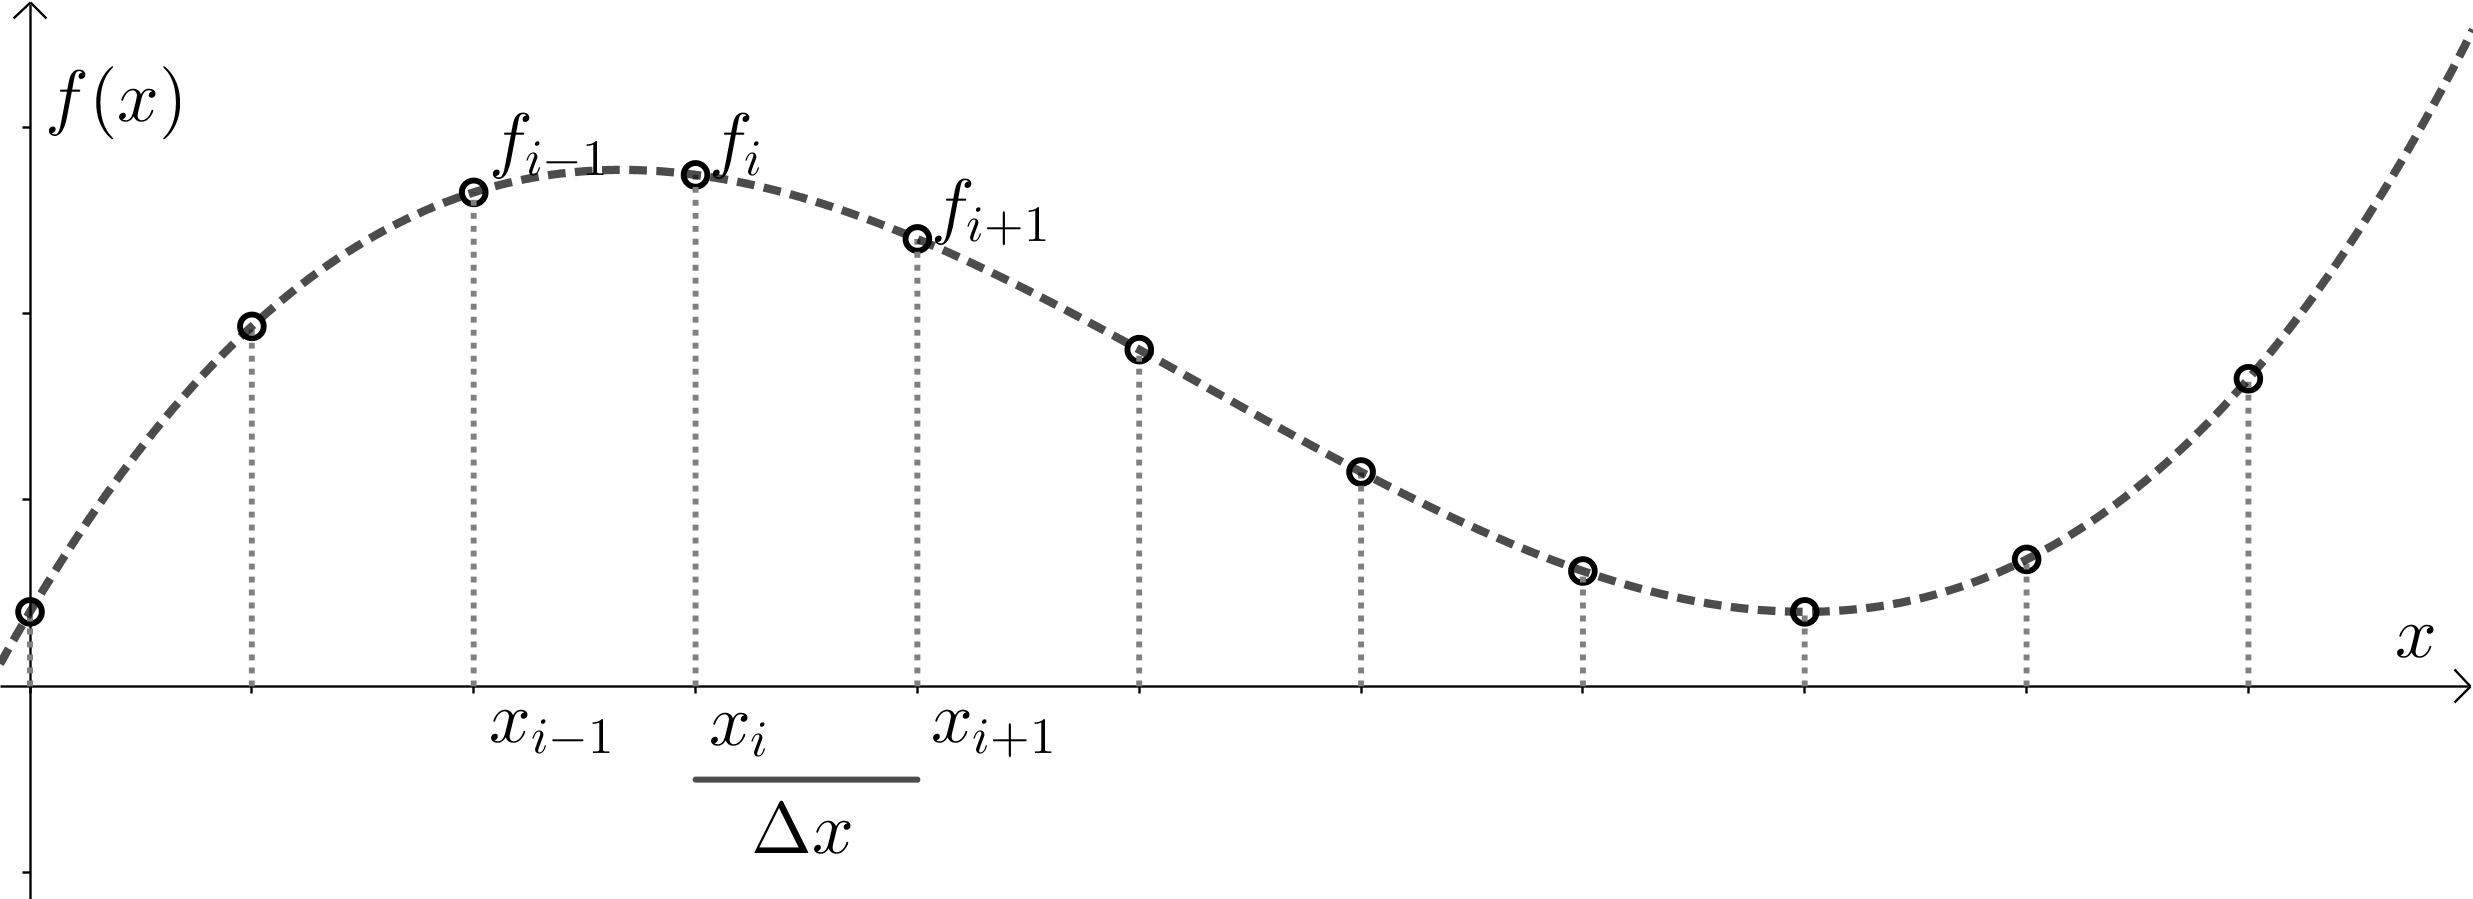
\includegraphics[width=\linewidth]{finite_difference1.png}
\end{figure}
With the $ x $-values given by:
\begin{equation}\label{key}
	x_i = x_0 + i \Delta x
\end{equation}
where $ x_0 $ is usually taken as the origin, for convenience. The sampled values of the system $ f(x_i) $ are then denoted in shorthand by
\begin{equation}\label{key}
	f_i \equiv f(x_i)
\end{equation}
This of course generalises to higher dimensional systems. For two dimensions we have $ y_j = y_0 + j \Delta y$, and $ f_{i,j} \equiv f(x_i, y_j) $, and more indices for even higher dimensions.

\section{L1A}
The idea behind the finite difference method is to replace all derivatives in the equations with differences instead. This can be seen as not letting the spacing $ h $ in the differential quotient go all the way to zero, but just to some small value. Since we are working with regular grids, a convenient value is the spacing between points $ \Delta x $:
\begin{equation}\label{key}
	\diff[d]{f(x_i)}{x} = \lim\limits_{h\to 0} \frac{f(x_i + h) - f(x_i)}{(x_i+h) - x_i} \to \frac{f(x_i + \Delta x) - f(x_i)}{\Delta x}
\end{equation}
In this particular case, the finite difference is called the ``forward difference'' (FD) since it uses the point of interest $ x_i $ and the one next to it $ x_{i+1} = x_i + \Delta x $. In the compact notation we have
\begin{equation}\label{key}
	\diff[d]{f_i}{x} \approx \frac{f_{i+1} - f_{i}}{\Delta x}
\end{equation}
There is also the ``backwards difference'' (BD):
\begin{equation}\label{key}
	\diff[d]{f_i}{x} \approx \frac{f_{i} - f_{i-1}}{\Delta x}
\end{equation}
And the ``central difference'' (CD):
\begin{equation}\label{key}
	\diff[d]{f_i}{x} \approx \frac{f_{i+1} - f_{i-1}}{2 \Delta x}
\end{equation}
These can be shown explicitly from the Taylor Polynomials for $ f(x) $ around $ x_i $. There are of course also higher order differences. In particular we use the second order central difference when studying the heat equation, as this includes a second derivative:
\begin{equation}\label{key}
	\diff[d]{^2 f_i}{x^2} \approx \frac{f_{i-1} - 2f_i + f_{i+1}}{\Delta x^2}
\end{equation}
This, however, only takes care of calculating derivatives. What we want is to follow the evolution of the system with time. This means we have to do some sort of numerical time integration as well. But that is the subject of next weeks hand-in.

There are some considerations we need to make when designing the simulation of the system. In general we have some restrictions in the form of time, memory and accuracy.

These restrictions boil down to choosing the parameters of the system (for example $ \Delta x $ and $ \Delta y $ so as to get an acceptable trade-off between the restrictions).

The first concern is accuracy. We set out to solve some partial differential equation. This is all for naught, if we do not calculate an accurate result. The easiest way of increasing the accuracy is to decrease the spacing between the nodes. This of course results in more accurate approximations of the derivatives (with analytical results as $ \Delta x \to 0 $), but also increases both computation time and memory cost (if we keep the domain constant).

One might then think, given infinite time and memory - could we just keep decreasing the grid spacing $ \Delta x $ to get a more accurate result? It turns out we cannot, as the computer cannot resolve the difference between values accurately, as they approach each other.

To be more specific, the computer stores the numbers as floating points numbers, which in Numpy has a spacing of $ 2.2204 \D 10^{-16} $ (called the machine epsilon) for double precision floats (accessed by \texttt{numpy.finfo(float).eps}). Two numbers which differ by less than this value will be identical to the computer, and their difference will thus be 0. Trying to then divide by this difference (for example) will lead to crashing of the simulation.

\section{Constructing the simulation}


When constructing the simulator it is useful to get a high-level overview of which values are needed to update each node. This is where the stencil comes in. This is is a schematic representation of which nodes are involved in each calculation. If, for example we want to calculate the second order derivative of a function at the point $ x_i $, using the second order centred difference, we will need the nodes $ x_i, x_{i+i} $ and $ x_{i-1} $. This can be graphically shown as
\begin{figure}[H]
	\centering
	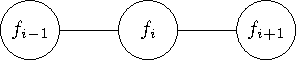
\includegraphics{stencil1.pdf}
\end{figure}
where each node is represented by a circle. Usually we denote the unknown in the system by $ u $ and reserve $ f $ for known functions, called the source terms.



\section{L1C}


\end{document}
